\documentclass{beamer}

\usepackage[latin1]{inputenc}
\usepackage{amsmath}
\usepackage{amssymb}
\usepackage{mathrsfs}
\usepackage{graphicx}
\usepackage{layout}
\usepackage{dsfont}
\usepackage[square,numbers,sort&compress]{natbib}
\usepackage[francais]{babel}
%\usepackage[top=2cm, bottom=3cm, left=2cm, right=2cm]{geometry}
\usepackage{listings}
\usepackage{algorithm}
\usepackage{algorithmic}
\usepackage{algorithmique}


\title{Soutenance stage L3 : Factorisation et calcul de logarithmes discrets : les algorithmes de crible}
\author{Oijid Nacim}
\institute{}
\usetheme{Warsaw}
\date{Septembre 2019}

%Macros
\newtheorem{defdef}{D�finition}
\newtheorem{nota}{Notation}
\newcommand{\p}{\mathbb{P}} 
\newcommand{\z}{\mathbb{Z}} 
\newcommand{\ztz}{$\mathbb{Z}/2\mathbb{Z}$} 
\newcommand{\al}{\alpha} 
\newcommand{\ere}{\textsuperscript{�re} }
\newcommand{\er}{\textsuperscript{er} }
\newcommand{\eme}{\textsuperscript{�me} }
\newcommand{\HRule}{\rule{\linewidth}{0.5mm}}


\begin{document}

\begin{titlepage}
 \begin{center}
  
\includegraphics[width = 20mm]{ENS_Lyon.png} \hfill
  
\includegraphics[width = 20mm]{cnrs.jpg} \hfill
  
\includegraphics[width = 20mm]{LIP.png}\hfill
  
\includegraphics[width = 20mm]{univ_lyon.jpg} \hfill
  
\includegraphics[width = 20mm]{ucbl.jpg}

\end{center}
\end{titlepage}

\section{Introduction}

\begin{frame}{Introduction}
  

  \begin{itemize}
  
\item<1,2,3,4> La cryptographie

 \item<2,3,4> RSA
  
  \item< 3,4> la place de la factorisation

 \item<4> Les algorithmes na�fs

  \end{itemize}
  
\end{frame}

\section{Le crible quadratique}

\subsection{Pr�sentation de l'algorithme}
\begin{frame}{Pr�sentation de l'algorithme}
    
\begin{itemize}

 
 \item<1, 2, 3> recherche exaustive des �ventuels petits facteurs
  
 \item<2, 3> Id�e : trouver $x$, $y$ tel que $x^2 \equiv y^2 [N]$, on aura alors $kN = (x-y)(x+y)$
 

 \item<3> D�composer en facteurs premiers les $x^2 - N$
 
 \item<3> Chercher une relation de d�pendance lin�aire
 
 
  \end{itemize}
  
\end{frame}

\subsection{Exemple}
\begin{frame}{Exemple}
    
\begin{itemize}

 
 \item<1, 2, 3> $N =$ 
  
 \item<2, 3> $ ^2 - N = $
 \item<2, 3> $ ^2 - N = $
 \item<2, 3> $ ^2 - N = $


 \item<3> Ce qui donne $ \equiv [N]$ donc $N = $  
 \end{itemize}
 \end{frame}
 
 \section{Le crible alg�brique}

\subsection{Lien avec le crible quadratique}
\begin{frame}{Lien avec le crible quadratique}
    
    
\begin{figure}
  \caption{Fonctionnement crible alg�brique.}
  \centering
  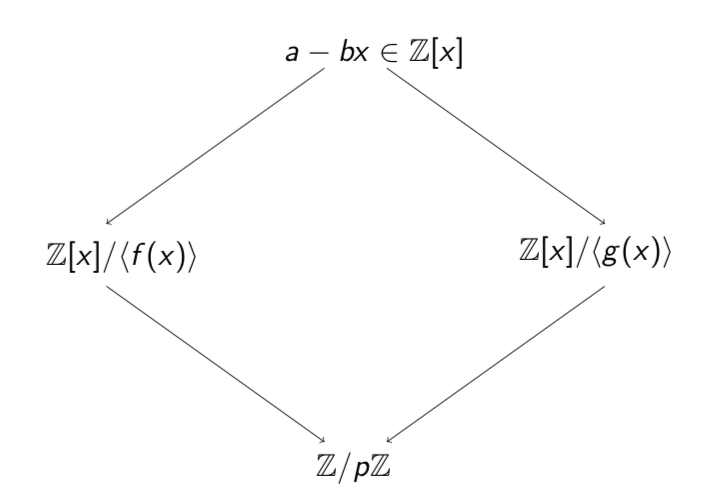
\includegraphics[width = 5 cm]{NFS1.png}
\end{figure}


\end{frame}

\subsection{Pr�sentation de l'algorithme}
\begin{frame}{Pr�sentation de l'algorithme}
    
\begin{itemize}

 
 \item<1, 2, 3, 4, 5> S�lection polynomiale
  \item <2, 3, 4, 5> Sp�cial-Qs
 \item<3, 4, 5> Crible
 \item<4, 5> Cofactorisation
 \item<5> Alg�bre lin�aire

 
  \end{itemize}
  
\end{frame}

 \section{Crible alg�brique : multi-sp�cial-Qs}

\subsection{La modification}
\begin{frame}{La modification}

\begin{itemize}
\item Un sp�cial-Q de chaque c�t� au lieu d'un seul.
\end{itemize}

\end{frame}

\subsection{R�sultats}
\begin{frame}{R�sultats}
    
\begin{itemize}

 
\item  
\end{itemize}
  
\end{frame}

\section{Conclusion}

\begin{frame}{Conclusion}
\center
Merci de votre attention !
\end{frame}


\end{document}



